\begin{frame}{TBB Partitioning} 
\todo{Fuse with following slide}
	\begin{itemize}
		\item tbb::parallel\_scan(..., partitioner)
		\item accepts auto\_ and simple\_partitioner
		\item tbb::parallel\_for(..., partitioner)
		\item accepts auto\_, simple\_, static\_ and affinity\_partitioner
	\end{itemize}
\end{frame} 

\begin{frame}{Partitioners:}
	\begin{itemize}
		\item auto\_partitioner: subdivides range in S subranges with S $\sim$ num\_threads further splitting occurs only when work stealing happens
		\item affinity\_partitioner: can be passed to several functions or loops indicating that the work should be split equally to earlier iterations or calls
		\item static\_partitioner: splits a range in S subranges with S = num\_threads
		\item simple\_partitioner: splits range recursively until not linger possible or grainsize is reached
	\end{itemize}
\end{frame}

\begin{frame}{Performance}
	\begin{figure}
		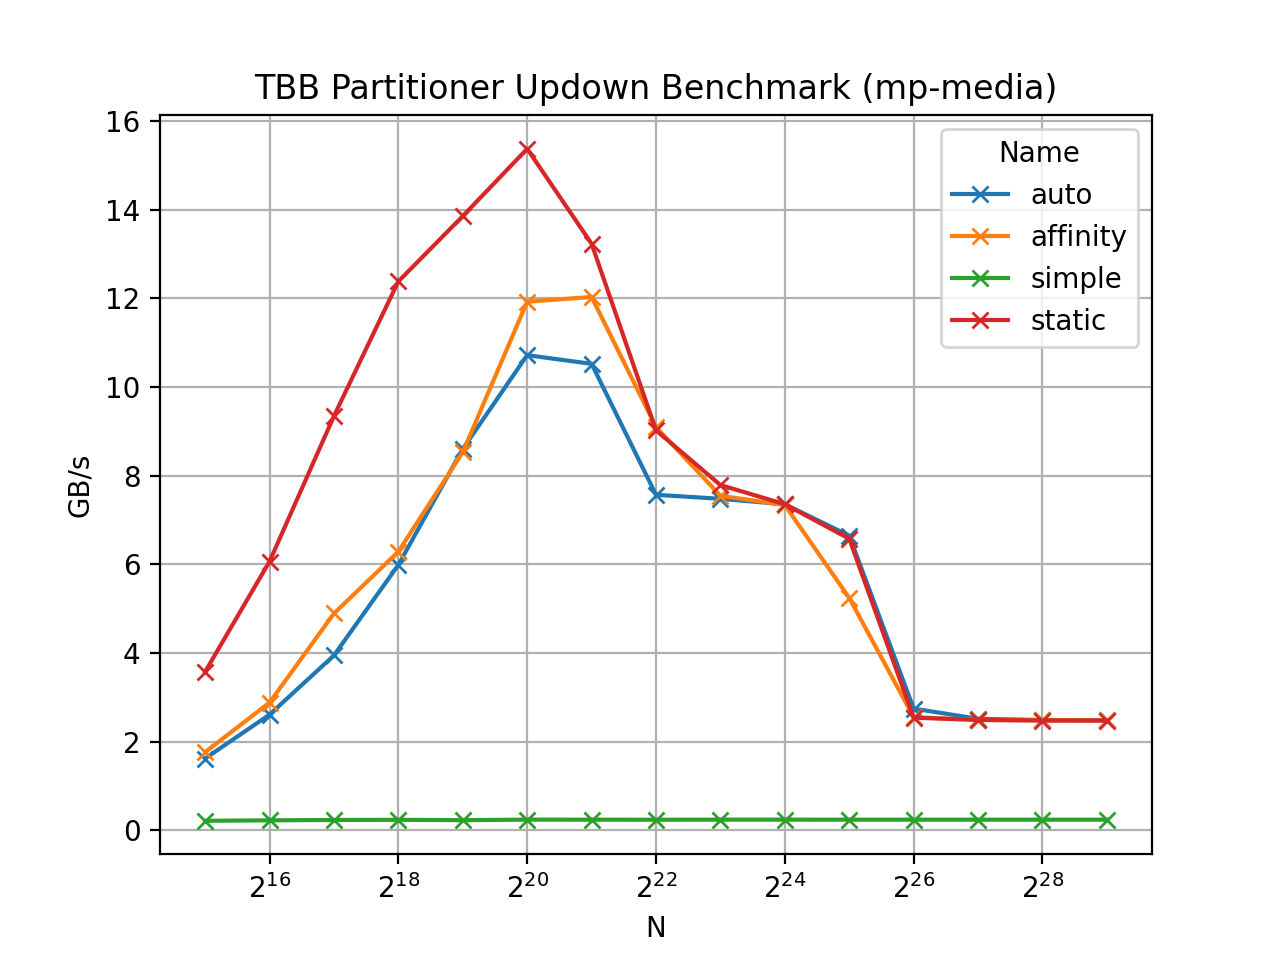
\includegraphics[width=80mm]{wiki/TBB Partitioner Updown Benchmark (mp-media).png}
		\caption{{partitioners on mp-media}}
	\end{figure}
\end{frame}

\begin{frame}{Performance}
	\begin{figure}
		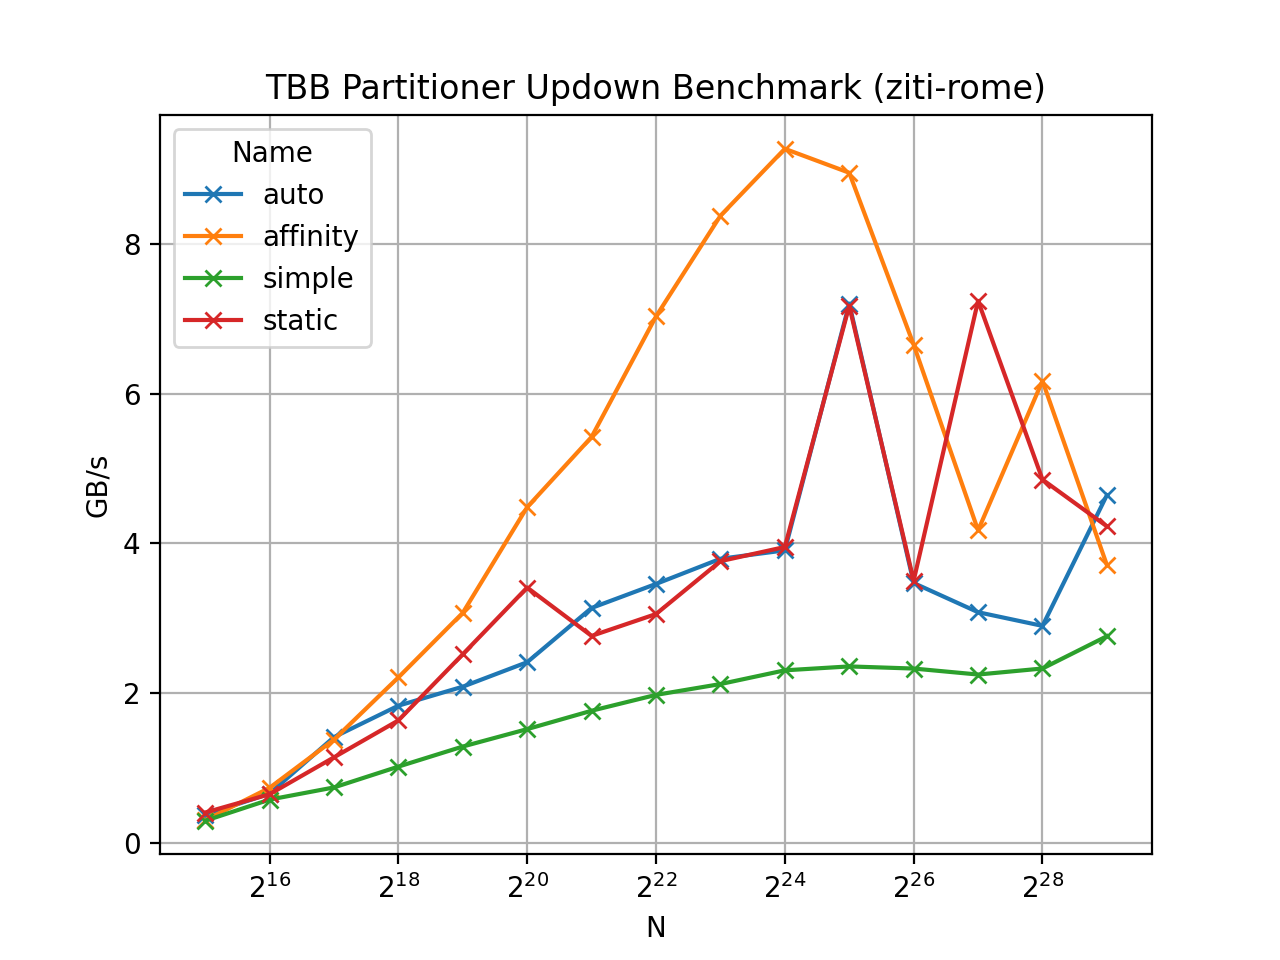
\includegraphics[width=80mm]{wiki/TBB Partitioner Updown Benchmark (ziti-rome).png}
		\caption{{partitioners on ziti-rome}}
	\end{figure}
\end{frame}
